% Chapter 1


\chapter{Einleitung} % Main chapter title

\label{Chapter1} % For referencing the chapter elsewhere, use \ref{Chapter1} 

%----------------------------------------------------------------------------------------

% Define some commands to keep the formatting separated from the content 
\newcommand{\keyword}[1]{\textbf{#1}}
\newcommand{\tabhead}[1]{\textbf{#1}}
\newcommand{\code}[1]{\texttt{#1}}
\newcommand{\file}[1]{\texttt{\bfseries#1}}
\newcommand{\option}[1]{\texttt{\itshape#1}}

%----------------------------------------------------------------------------------------

\section{Aufbau der Arbeit}\label{Aufbau der Arbeit}
Im Rahmen dieser Arbeit wollen wir ermöglichen parallele Datenbankprozesse sowohl zu analysieren als auch zu Transformieren. Um zu verstehen was genau hier passieren soll und wie eine Mögliche Umsetzung aussehen könnte, müssen wir zunächst einige Begriffe definieren und deren Bedeutung verstehen.\\
Da wir uns im generellen Bereich von Prozessen befinden, muss zunächst erläutert werden was unter einem Prozess zu verstehen ist und auf welche Art von Prozessen wir uns beschränken wollen.
Bei Prozessen handelt es sich um sogenannte \textit{reaktive Systeme}. Es sind also Systeme, welche auf eine Eingabe warten und je nach Zustand entsprechend reagieren. Hierfür sind in jedem erdenklichen Teil des Alltags Beispiele zu finden. Es kann sich um Komplexe Prozesse in Computerspielen oder Betriebssystemen handeln, oder auch um ganz einfache Abläufe im Alltag. Ein einfaches Beispiel ist in Abbildung \ref{Alltag} dargestellt. Hier ist der Tagesablauf eines gewöhnlichen Angestellten einer beliebigen Firma zu sehen.\\
Wir wollen uns in dieser Arbeit zum größten Teil mit Abläufen von Geschäftsprozessen auseinandersetzen. Damit sind unter anderem jene Abläufe gemeint, die innerhalb von beispielsweise Firmen passieren. Es kann sich hier um viele Verschiedene Abläufe handeln.\\
Ein passendes Beispiel ist in Abbildung \ref{ersteReg} zu sehen. Es handelt sich hier um einen Prozess, welcher auf einer beliebigen Internetseite abläuft. Wir beschränken uns hier der Einfachheit halber auf den Prozess des Erstellens eines Accounts. Also auf den Registrierungsprozess. In unserem Beispiel muss der Nutzer auf der Homepage zunächst den Button „Registrieren“ drücken. Er wird im Anschluss auf die korrekte Internetseite weitergeleitet und hat da die Möglichkeit seine Anmeldedaten anzugeben. Nun muss die Korrektheit der Daten geprüft werden. Im Anschluss wird der Nutzer erstellt und wieder auf die Homepage zurück geleitet.\\
\begin{figure}
\centering
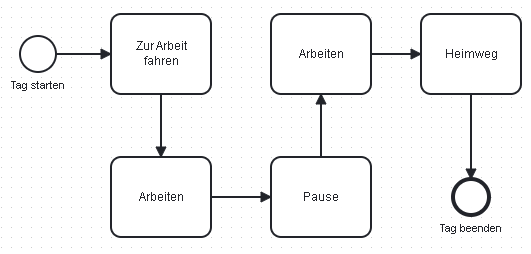
\includegraphics[scale=0.7]{Figures/Einleitungbsp1}
\decoRule
\caption[Alltag eines Mitarbeiters]{Alltag eines Mitarbeiters}
\label{Alltag}
\end{figure}\begin{figure}
\centering
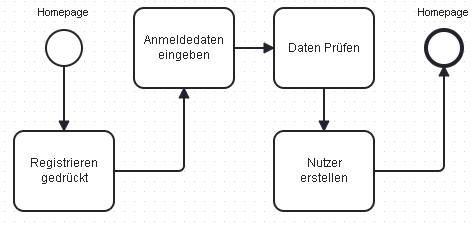
\includegraphics[scale=0.7]{Figures/Einleitungbsp2}
\decoRule
\caption[Einfacher Registrierungsprozess]{Einfacher Registrierungsprozess}
\label{ersteReg}
\end{figure}Solche und ähnliche Prozesse laufen in jeder erdenklichen Firma ab und unterscheiden sich sehr stark voneinander in Komplexität und Inhalt.\\
Bei dem zweiten Begriff, der verstanden werden muss handelt es sich um BPMN (Business Proccess Moddeling Notation). Hierbei handelt es sich um eine Standardisierte Modellierungssprache. Die in den Abbildungen \ref{Alltag} und  \ref{ersteReg} dargestellten Beispiele wurden bereits in BPMN dargestellt. Eine Detailliertere Beschreibung erfolgt im Abschnitt \ref{BPMN} doch die wichtigsten Features sollen hier schon einmal erwähnt werden. Sie sind, neben den Aktivitäten, welche durch abgerundete Rechtecke dargestellt werden und der Konkatenation dieser Aktivitäten durch die Pfeile, die sogenannten Gateways, welche durch Rauten mit einem Entsprechenden Symbol dargestellt werden. Ist ein \textit{X} in die Raute geschrieben so handelt es sich um ein Exklusives OR-Gateway. Hier kann exakt eine der folgenden Pfade ausgeführt werden. Ist ein \textit{+} in die Raute geschrieben, so liegt ein paralleles Gateway vor. Hier werden alle Pfade gleichzeitig ausgeführt. Ein weites paralleles Gateway vereinigt die Pfade dann wieder. An dieser Stelle wird also gewartet, bis alle parallelen Aktivitäten durchgeführt worden sind. Diese Arbeit beschäftigt sich ausschließlich mit Prozessen in BPMN. Es wird allerdings nur eine Teilmenge benutzt.\\
Zuletzt muss nun noch erläutert werden zu was diese Prozesse transformiert werden sollen. Hierzu müssen wir den Begriff einer Prozessalgebra genauer erläutern. Bei einer Prozessalgebra handelt es sich nun um einen mathematischen Kernkalkül zur Darstellung von Prozessen. Es bietet also eine Möglichkeit die selben Prozesse durch eine Art Formeln darzustellen. Wir wollen in dieser Arbeit eine Prozessalgebra verwenden, welche auf ACP basiert. ACP ist kurz für \textit{Algebra of Communicating Processes.} Zum besseren Verständnis möchte ich auch hier die wichtigsten Features von ACP erläutern. Ähnlich zu BPMN gibt es Möglichkeiten zur Darstellung von Konkatenation, oder-Zweigen und auch Parallelen Zweigen. Eine Aktivität wird durch einfach als Variable dargestellt. Wie diese genannt wird, ist zunächst irrelevant. Eine Konkatenation wird durch ein \textit{*} dargestellt. Ein Exklusiver oder-Zweig wird durch ein \textit{+} und ein paralleler Zweig durch \textit{||} dargestellt. Würde man das Beispiel in Abbildung  \ref{ersteReg} also nun nach ACP überführen, so würde ein Mögliches Ergebnis wie folgt aussehen:\\
$P:=Start*RegestrierenGedrueWckt*AnmeldeDatenEingeben*DatenPruefen*NutzerErstellen*Homepage $

\section {Ziel der Arbeit}\label {Ziel der Arbeit}
Das Ziel dieser Arbeit ist es nun Programm zu entwickeln, welches ein BPMN Diagramm einlesen und dieses zu einer Formel in der Prozessalgebra überführen kann. Es soll also ein Mapping von BPMN nach ACP erfolgen.\\
Der Zweck dieser Arbeit wird erkennbar, sobald Daten in form einer relationalen Datenbank für den Prozess relevant werden. BPMN bietet hier nur schwammige und unübersichtliche Methoden die Daten darzustellen. Es erweist sich also als schwierig zu Analysieren und zu verifizieren, was genau mit den Daten passiert. Zudem lässt BPMN zu viel Raum für Interpretation. Es wird viel mit Kommentaren gearbeitet und was genau in einem bestimmten Abschnitt des Prozesses passiert ist in vielerlei Hinsicht offen zur Interpretation. ACP ist etwas Strukturierter. Zudem bietet die Variante die von uns genutzt wird die Möglichkeit mit einer konkreten Datenbank zu kommunizieren und Anweisungen auf dieser auszuführen. Aus diesem Grund ist ein weiteres Ziel dieser Arbeit, die passenden Datenbankanweisungen zu dem jeweiligen Prozess auf einer relationalen Datenbank auszuführen.




